% !TeX root = ../../main.tex
% Add the above to each chapter to make compiling the PDF easier in some editors.

\section{Survey Evaluation}\label{ord:ch5:sec4_survey}
% RE-1469
After participating in the benchmark study 17 users also filled out the post survey.
This survey consists out of five questions, to gain deeper insights on the user's experience.
The questions and their results are presented in \ref{fig:ch5:sec4:suvery}.
% Soft Factors
% Useability

\begin{figure}
	\centering
	\begin{subfigure}[t]{0.48\textwidth}
		\centering
		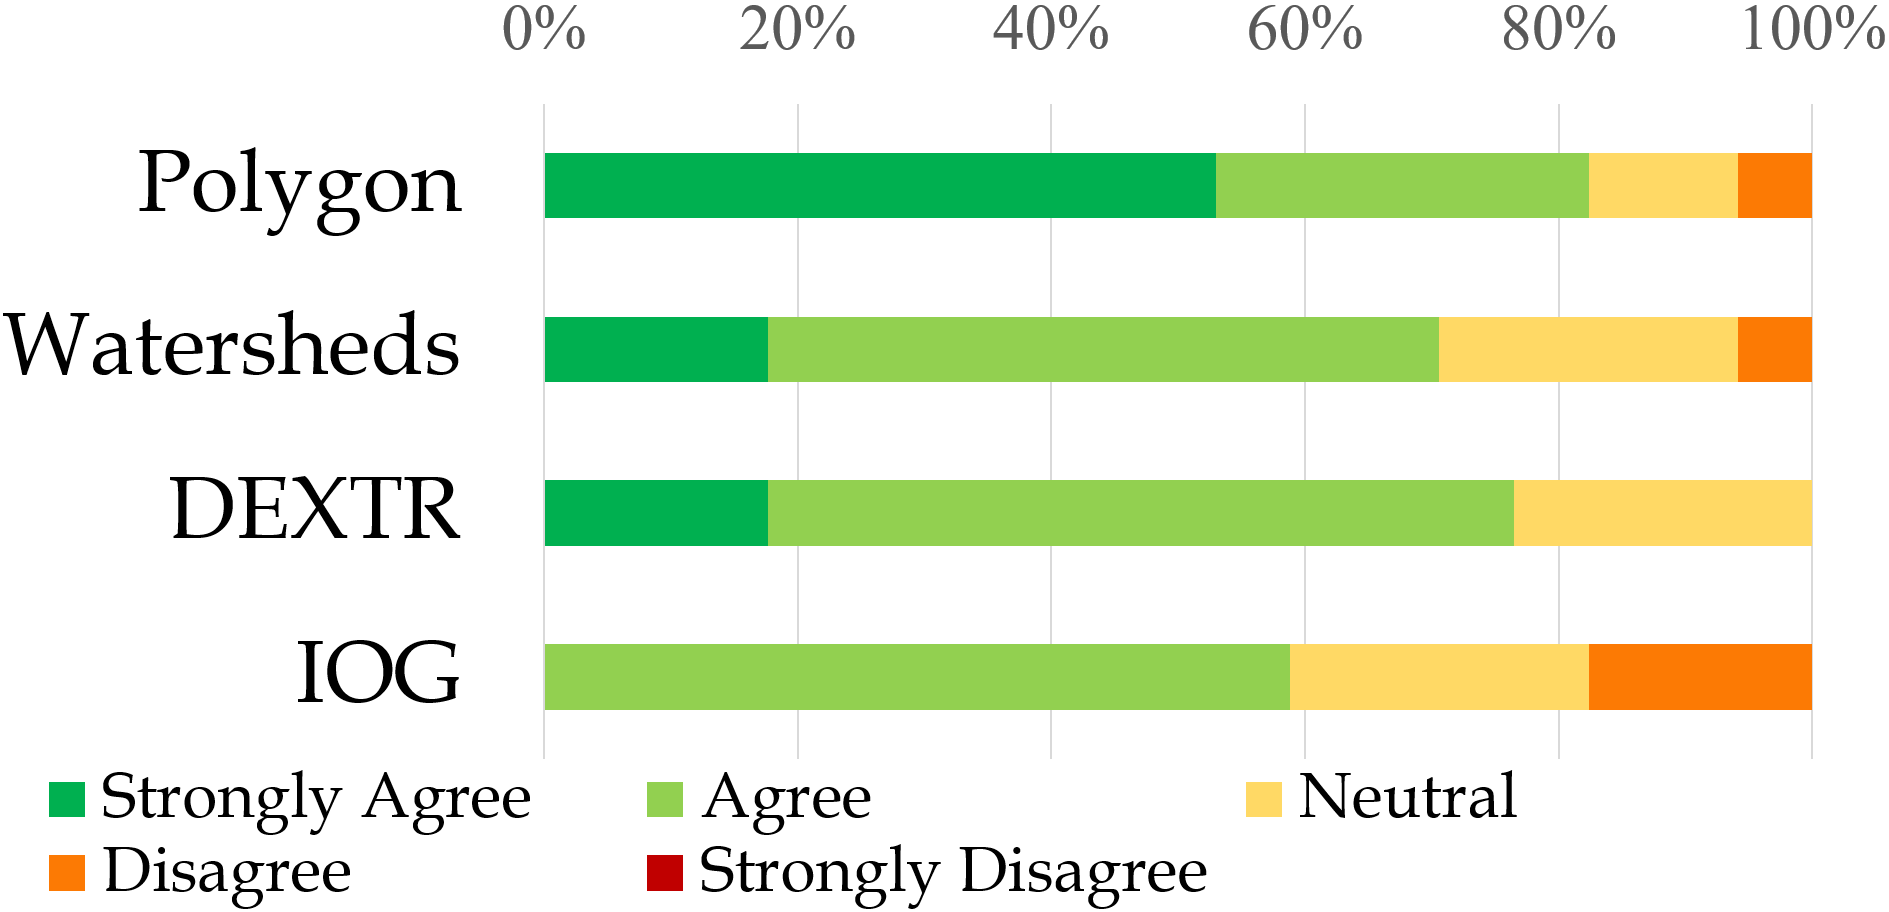
\includegraphics[width=\textwidth]{figures/chap54_q1.png}
		\caption{
			Question 1: \textit{The result / prediction masks of the method were as I expected them to be.}
		} \label{fig:ch5:sec4:q1}
	\end{subfigure}
	\hfill
	\begin{subfigure}[t]{0.48\textwidth}
		\centering
		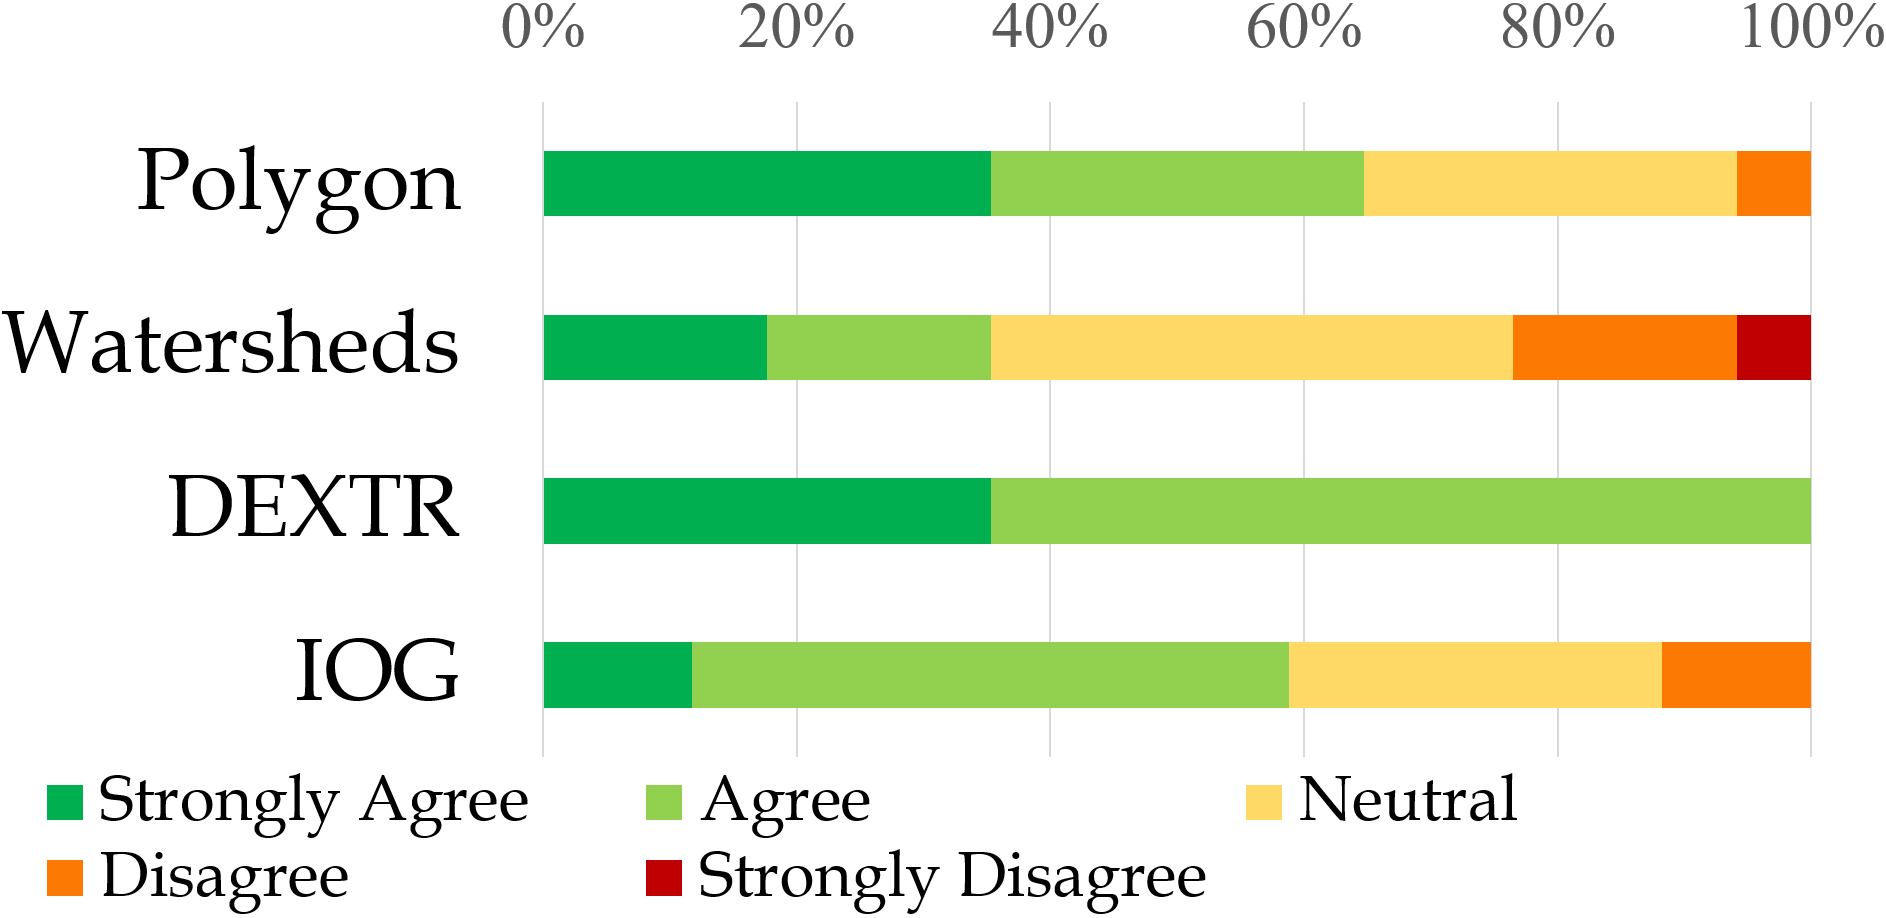
\includegraphics[width=\textwidth]{figures/chap54_q2.png}
		\caption{
			Question 2: \textit{I was satisfied with the result / prediction masks.}
		} \label{fig:ch5:sec4:q2}
	\end{subfigure}
	\\
	\begin{subfigure}[t]{0.48\textwidth}
		\centering
		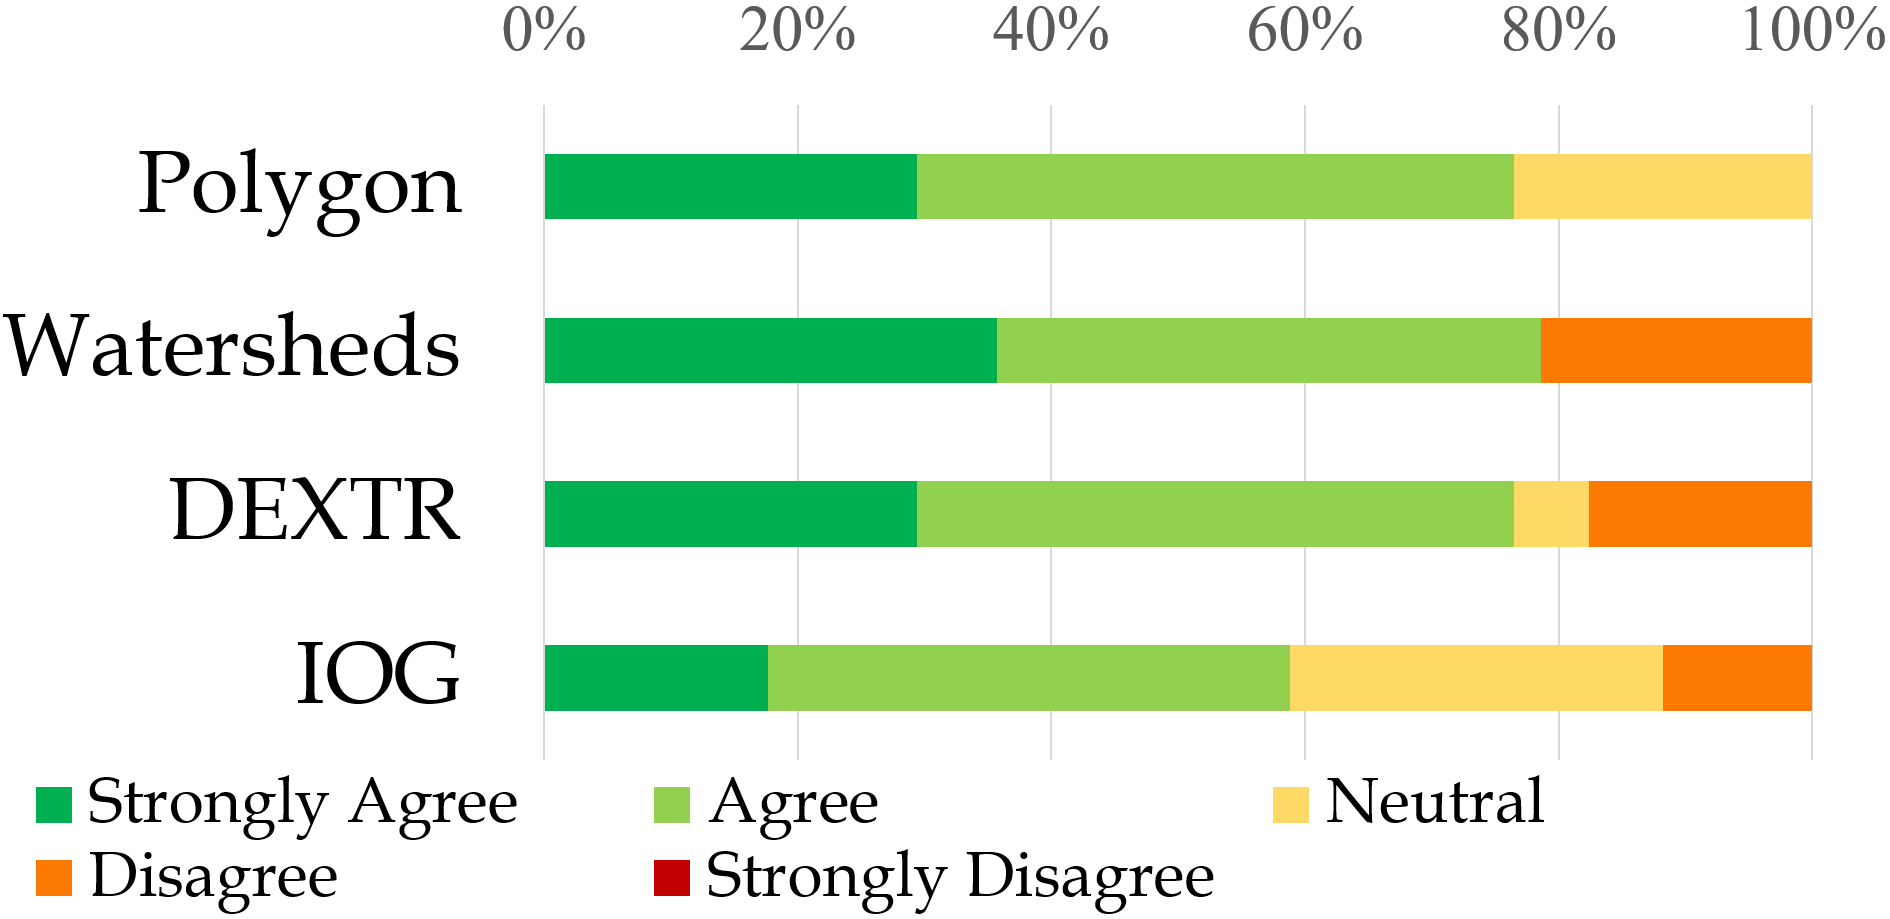
\includegraphics[width=\textwidth]{figures/chap54_q3.png}
		\caption{
			Question 3: \textit{With more experience / time in the labeltool I became better at handling the method and applying it.}
		} \label{fig:ch5:sec4:q3}
	\end{subfigure}
	\hfill
	\begin{subfigure}[t]{0.48\textwidth}
		\centering
		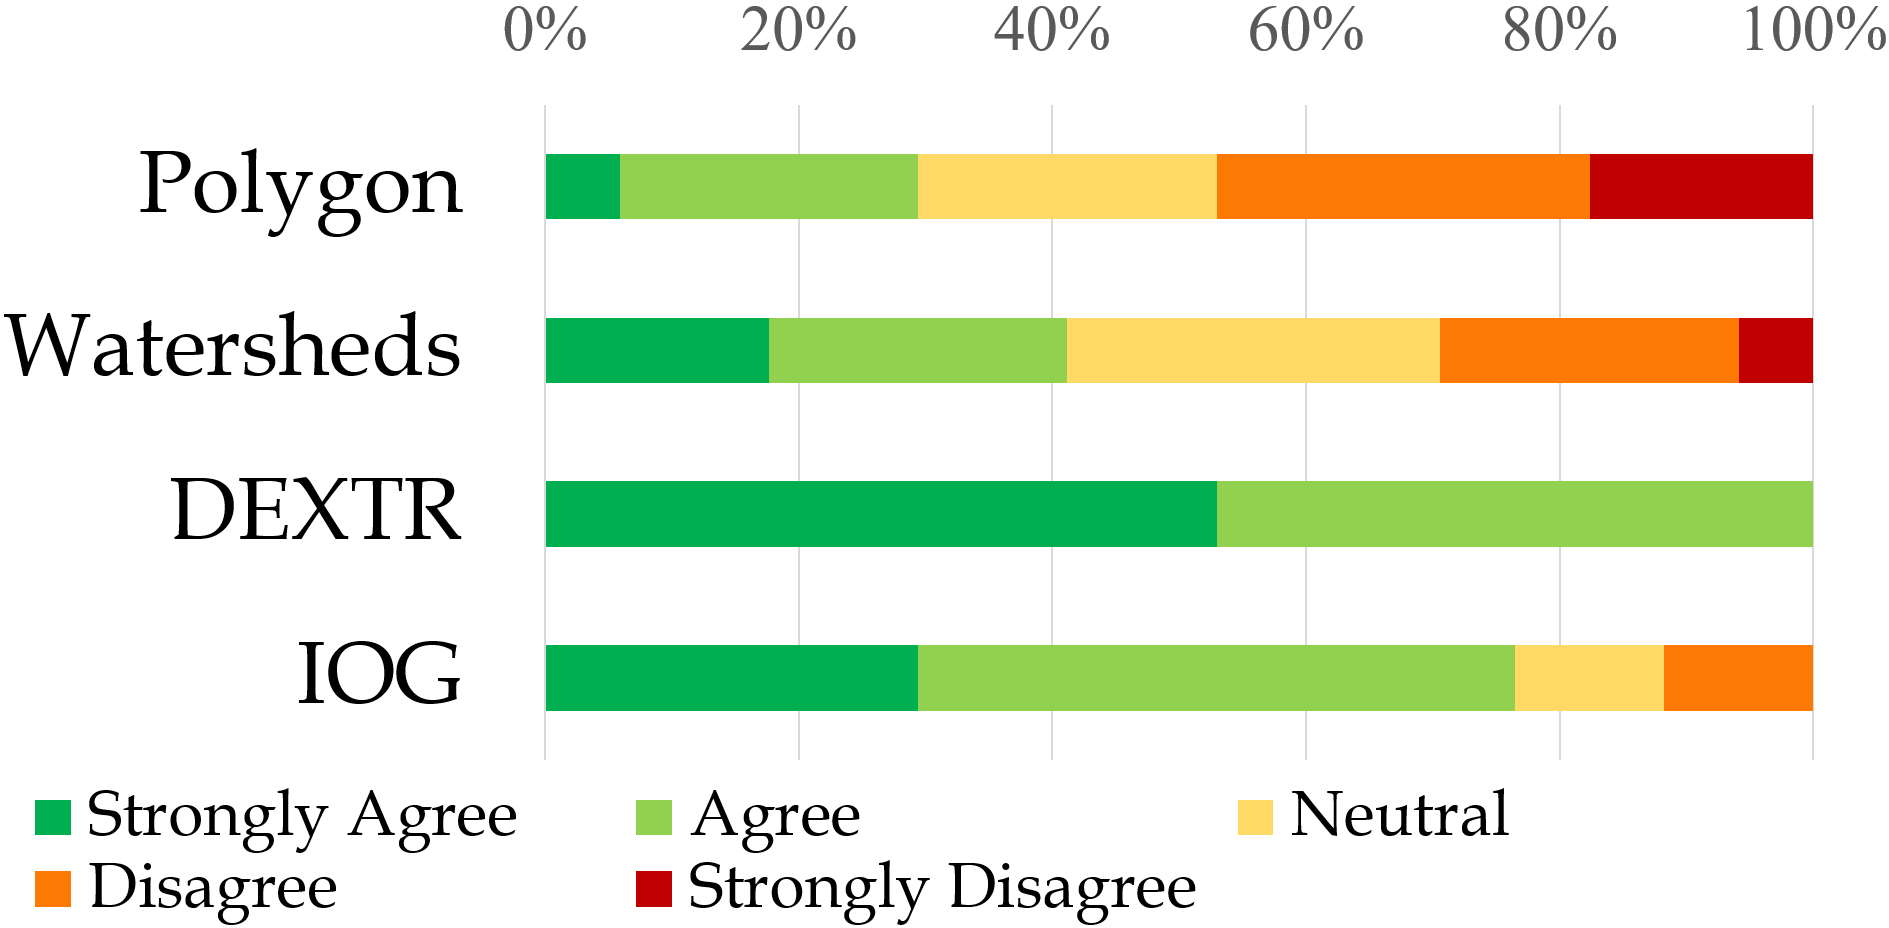
\includegraphics[width=\textwidth]{figures/chap54_q5.png}
		\caption{
			Question 4: \textit{It was ‘fun’ / ‘exciting’ to use the method.}
		} \label{fig:ch5:sec4:q4}
	\end{subfigure}
	\\
	\begin{subfigure}[t]{0.48\textwidth}
		\centering
		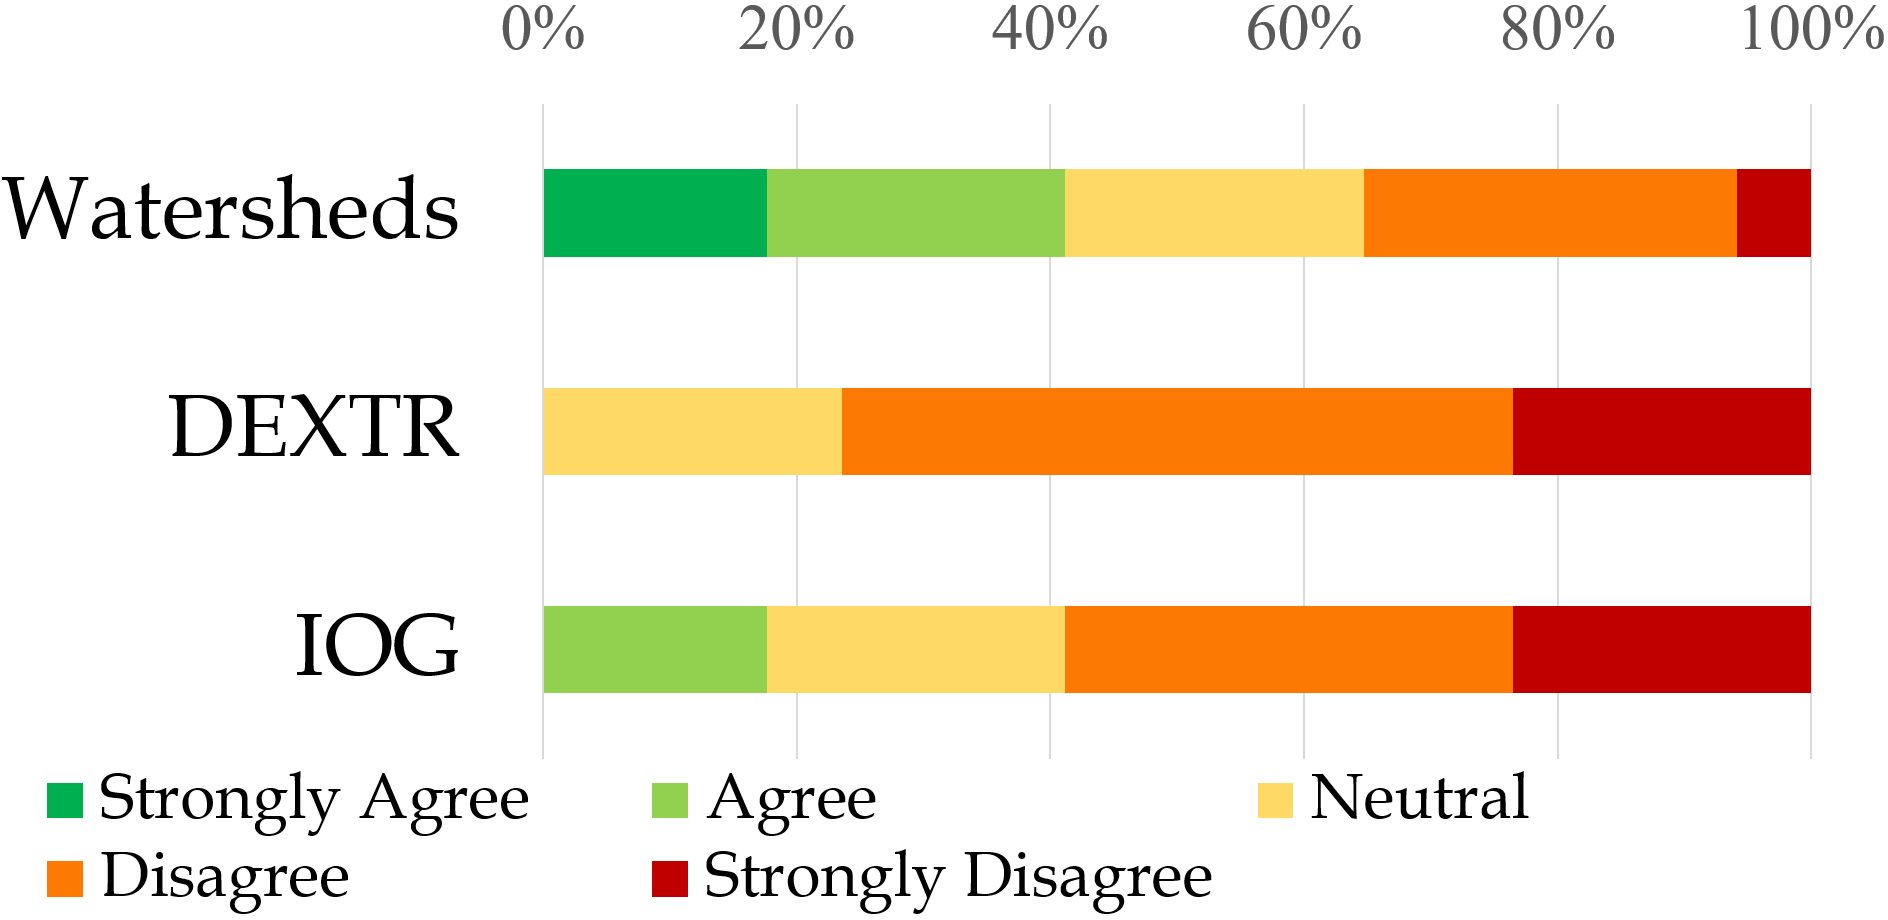
\includegraphics[width=\textwidth]{figures/chap54_q4.png}
		\caption{
			Question 5: \textit{By manually drawing a polygon I could achieve a better result in the same time.}
		} \label{fig:ch5:sec4:q5}
	\end{subfigure}
	\caption [Watershed User Interaction]{
		Responses on the questions from the survey.
		The answer options for all question are \textit{Strongly Agree}, \textit{Agree}, \textit{Neutral}, \textit{Disagree}, and \textit{Strongly Disagree}.
	} \label{fig:ch5:sec4:suvery}
\end{figure}
% TODO update proper figure if approved

In order to be accepted by an user a method needs to be understandable and create deterministic results.
When the method performs as intended, a pleasant user experience is created, while frustration is caused otherwise.
These factors are investigated in the questions one and two, which represent that all methods perform as the user expects and the users are mostly satisfied with the result.

Further, in question 3 and 5 it was researched whether the user was time efficient and improved over time.
A review of the total experience and the pleasantly of the application is asked in Question 4.
Here the \gls{dl} based methods received good feedback.
This reasons in their little user interaction and excitement of applying novel methods.

In conclusion, based on this survey the \gls{dextr} method seems to provide the best user experience.
Manual methods like polygon drawing or Watersheds also serve good results, but are not time efficient and pleasant to apply, compared to the \gls{dextr} and \gls{iog} method.  
